%\documentclass{beamer}
\documentclass[handout]{beamer}
% This file is a solution template for:

% - Giving a talk on some subject.
% - The talk is between 15min and 45min long.
% - Style is ornate.

% Copyright 2004 by Till Tantau <tantau@users.sourceforge.net>.
%
% In principle, this file can be redistributed and/or modified under
% the terms of the GNU Public License, version 2.
%
% However, this file is supposed to be a template to be modified
% for your own needs. For this reason, if you use this file as a
% template and not specifically distribute it as part of a another
% package/program, I grant the extra permission to freely copy and
% modify this file as you see fit and even to delete this copyright
% notice. 


\mode<presentation>
{
  \usetheme{Montpellier}

  %\setbeamercovered{transparent}
  % or whatever (possibly just delete it)
}

\usepackage{xmpmulti} % package that defines \multiinclude

\usepackage[english]{babel}

\usepackage[latin1]{inputenc}

\usepackage{times}
\usepackage[T1]{fontenc}
% Or whatever. Note that the encoding and the font should match. If T1
% does not look nice, try deleting the line with the fontenc.

\title [Specialists] %(optional, use only with long paper titles)
{Predictors that Specialize}

\author[Freund] % (optional, use only with lots of authors)
{Yoav Freund}
% - Give the names in the same order as the appear in the paper.
% - Use the \inst{?} command only if the authors have different
%   affiliation.

\institute[Universities of Somewhere and Elsewhere] % (optional, but mostly needed)

\subject{Machine Learning}
% This is only inserted into the PDF information catalog. Can be left
% out. 

% If you have a file called "university-logo-filename.xxx", where xxx
% is a graphic format that can be processed by latex or pdflatex,
% resp., then you can add a logo as follows:

% \pgfdeclareimage[height=0.5cm]{university-logo}{university-logo-filename}
% \logo{\pgfuseimage{university-logo}}



% Delete this, if you do not want the table of contents to pop up at
% the beginning of each subsection:
%% \AtBeginSubsection[]
%% {
%%   \begin{frame}<beamer>
%%     \frametitle{Outline}
%%     \tableofcontents[currentsection,currentsubsection]
%%   \end{frame}
%% }


% If you wish to uncover everything in a step-wise fashion, uncomment
% the following command: 

\beamerdefaultoverlayspecification{<+->}

\newcommand{\newmcommand}[2]{\newcommand{#1}{{\ifmmode {#2}\else\mbox{${#2}$}\fi}}}
\newcommand{\renewmcommand}[2]{\renewcommand{#1}{{\ifmmode {#2}\else\mbox{${#2}$}\fi}}}
\newcommand{\newmcommandi}[2]{\newcommand{#1}[1]{{\ifmmode {#2}\else\mbox{${#2}$}\fi}}}
\newcommand{\newmcommandii}[2]{\newcommand{#1}[2]{{\ifmmode {#2}\else\mbox{${#2}$}\fi}}}
\newcommand{\newmcommandiii}[2]{\newcommand{#1}[3]{{\ifmmode {#2}\else\mbox{${#2}$}\fi}}}

\newcommand{\algfnt}{\bf}

\newmcommand{\ouralg}{{\mbox{\algfnt Hedge}({\eta})}}

\newmcommand{\iter}{T}

\newfont{\cmmib}{cmmib10}
\newcommand{\boldell}{{\mbox{\cmmib \symbol{'140}}}}


\newmcommandi{\costvec}{{\boldell}^{#1}}
\newmcommandii{\cost}{{\ell}^{#1}_{#2}}

\newmcommandi{\rd}{\tilde{#1}}

\newmcommandi{\distvec}{{\bf p}^{#1}}
\newmcommandi{\rddistvec}{\rd{\bf p}^{#1}}
\newmcommandii{\dist}{{p}^{#1}_{#2}}
\newmcommandii{\rddist}{\rd{p}^{#1}_{#2}}

\newmcommandi{\bdistvec}{{\bf q}^{#1}}
\newmcommandii{\bdist}{{q}^{#1}_{#2}}

\newmcommandi{\wtvec}{{\bf w}^{#1}}
\newmcommandi{\rdwtvec}{\rd{\bf w}^{#1}}
\newmcommandii{\wt}{{w}^{#1}_{#2}}
\newmcommandii{\rdwt}{\rd{w}^{#1}_{#2}}


\newcommand{\Nweight}[2]{V_{#1}^{#2}}	%the normalized weight
\newcommand{\dweight}[2]{w^{#2}(#1)} % initial density measure
\newcommand{\TEloss}[1]{L_{#1}}	%total loss of expert i
\newcommand{\BEloss}{L_{\min}}	%total loss of the best expert
\newcommand{\TAloss}{L_A}	%total loss of algorithm
\newcommand{\weight}[2]{W_{#1}^{#2}} % weight assigned to expert
\newcommand{\btheta}{\hat{\theta}}

\newcommand{\R}[1]{{\color{red}{#1}}}
\newcommand{\B}[1]{{\color{blue}{#1}}}
\newcommand{\RM}[1]{{\color{red}{$#1$}}}


%BANDITS
\newcommand{\Aplay}{{\bf Hedge}}
\newcommand{\Aest}{{\bf Exp3}}
\newcommand{\Aesthp}{{\bf Exp3.P}}
\newcommand{\Aestg}{{\bf Exp3.P.1}}
\newcommand{\Aests}{{\bf Exp3.S}}
\newcommand{\Aessg}{{\bf Exp3.S.1}}
\newcommand{\Astrat}{{\bf Exp4}}
\newcommand{\Abound}{{\bf Exp3.1}}
\newcommand{\Gbest}{G_{\rm max}}

\newcommand{\defeq}{\stackrel{\rm def}{=}}
\newcommand{\compl}{\mbox{\sc h}}
\newcommand{\theset}[2]{\{ {#1} \,:\, {#2} \}}

\newmcommandii{\stratv}{\mbox{\boldmath $\xi$}^{#1}({#2})}

%Games paper
\newmcommand{\M}{\bf M}
\newmcommand{\dM}{\M'}
\newmcommand{\Row}{\bf R}
\newmcommand{\dRow}{\R'}
\newmcommand{\C}{\bf C}
\newmcommand{\dC}{\C'}
\newmcommand{\D}{D}
\renewmcommand{\P}{\bf P}
\newmcommand{\Q}{\bf Q}
\newmcommand{\Dt}{\D_t}
\newmcommand{\Pt}{\P_t}
\newmcommand{\Qt}{\Q_t}
\newmcommand{\Pstar}{\P^*}	% the min/max optimal mixed strategy
\newmcommand{\Pref}{\tilde{\P}}	% a reference mixed strategy (not
				% necessarily min/max)
\newmcommand{\Qstar}{\Q^*}
\newmcommand{\Pa}{\overline{\P}}
\newmcommand{\Qa}{\overline{\Q}}
\newmcommand{\Qh}{\hat{\Q}}
\newmcommandi{\trans}{{#1}^{\rm T}}
\newmcommand{\mhx}{\M(h,x)}
\newmcommand{\mxh}{\dM(x,h)}
\newmcommand{\mpq}{\M(\P,\Q)}
\newmcommand{\mpsq}{\M(\Pstar,\Q)}
\newmcommand{\mpsqt}{\M(\Pstar,\Qt)}
\newmcommand{\mptqt}{\M(\Pt,\Qt)}
\newmcommand{\mptt}{\M(\Pt,t)}
\newmcommand{\mptq}{\M(\Pt,\Q)}
\newmcommand{\mpqt}{\M(\P,\Qt)}
\newcommand{\minp}{\min_{\P}}
\newcommand{\maxq}{\max_{\Q}}
\newcommand{\RE}[2]{{\rm RE}\left( {#1} \; \parallel \; {#2} \right) }

\newmcommand{\sumt}{\sum_{t=1}^T}
\newmcommand{\sumin}{\sum_{i=1}^n}
\newmcommand{\delt}{\Delta_{T,n}}
\newcommand{\nextline}{\vspace{0.2cm}\\}   % a little space for equation arrays

\newcommand{\lwalg}{\mbox{\rm MW}}
\newcommand{\lwalgvar}{\mbox{\rm vMW}}

%%
\newcommand{\E}{\mbox{\rm\bf E}}
\newcommand{\p}[2]{p_{#1}(#2)}
\newcommand{\q}[2]{q_{#1}(#2)}
\newcommand{\x}[2]{x_{#1}({#2})}
\newmcommand{\bx}{\mbox{\boldmath$x$}}
\newmcommandi{\xv}{\bx({#1})}
\newmcommand{\xvt}{\xv{t}}
%\newcommand{\w}[2]{w_{#1}({#2})} replaced by \wt, but remember to switch order of parameters i and t
\renewcommand{\i}[1]{i_{#1}}
\newcommand{\hx}[2]{\hat{x}_{#1}(#2)}
\newcommand{\hxit}{\hx{\i{t}}{t}}
\newcommand{\pit}{\p{\i{t}}{t}}
\newcommand{\xit}{\x{\i{t}}{t}}
\newcommand{\expb}[1]{\exp\left(#1\right)}

\newcommand{\vp}{{\mathbf p}}
\newcommand{\vu}{{\mathbf u}}
\newcommand{\vv}{{\mathbf v}}
\newcommand{\vx}{{\mathbf x}}
\newcommand{\vy}{{\mathbf y}}

\newcommand{\HedgeLoss}{L_{\mbox{\footnotesize Hedge}}}

\newcommand{\W}{\vec{W}}
\newcommand{\V}{\vec{V}}
\newcommand{\X}{\vec{X}}
\newcommand{\vb}{\vec{b}}
%\newcommand{\loss}{\vec{\ell}}
\newcommand{\loss}{L}
%\newcommand{\elloss}[2]{\ell_{#1}^{#2}} %loss of expert i at time t
\newcommand{\elloss}[2]{\ell_{#2}\left( #1 \right)} %loss of expert i at time t
\newcommand{\w}[1]{\makebox[12pt]{{#1}}}
\newcommand{\Rps}{\mbox{\tt R}}
\newcommand{\rPs}{\mbox{\tt P}}
\newcommand{\rpS}{\mbox{\tt S}}
\newcommand{\rpstie}{\w{$\frac{1}{2}$}}
\newcommand{\rpswin}{\w{$0$}}
\newcommand{\rpsloss}{\w{$1$}}

\newmcommand{\decspace}{\Delta}
\newmcommand{\decsym}{\delta}
\newmcommandi{\dec}{\decsym^{#1}}
\newmcommand{\decdistsym}{\cal D}
\newmcommandi{\decdist}{{\decdistsym}^{#1}}

\newmcommand{\simpdistspace}{{\bf \cal S}}
\newmcommand{\domset}{{\rm dom}(\decdistsym)}

\newmcommand{\expdistsym}{{\cal E}}
\newmcommandii{\expdist}{{\expdistsym}^{#1}_{#2}}
\newmcommand{\expdecsym}{{\varepsilon}}
\newmcommandii{\expdec}{\expdecsym^{#1}_{#2}}

\newmcommand{\outspace}{\Omega}
\newmcommand{\outsym}{\omega}
\newmcommandi{\out}{\outsym^{#1}}

%\newmcommandii{\Dkl}{D_{\mbox{kl}}\paren{#1||#2}}
\newmcommandii{\Dkl}{{\rm {KL}}\paren{{#1}\;||\;{#2}}}

\newmcommandi{\sumwts}{\sum_{i=1}^N \wt{#1}{i}}

\newmcommand{\lossalg}{L_A}
\newmcommand{\lossouralg}{{L_{\mbox{\scriptsize\algfnt Hedge}(\eta)}}}
\newmcommand{\lossS}{{L_{\mbox{\scriptsize\algfnt S}}}}
\newmcommandi{\lossi}{L_{#1}}
\newmcommandii{\lossit}{L_{#1}^{#2}}

\newmcommandi{\upbnd}{\tilde{#1}}

\newcommand{\angles}[1]{{\left\langle {#1} \right\rangle}}
\newcommand{\paren}[1]{{\left( {#1} \right)}}
\newcommand{\brac}[1]{{\left[ {#1} \right]}}
\newcommand{\braces}[1]{{\left\{ {#1} \right\}}}

\newcommand{\abs}[1]{{\left| {#1} \right|}}
\newcommand{\ceiling}[1]{{\left\lceil {#1} \right\rceil}}

\newfont{\msym}{msbm10}
\newcommand{\real}{\mbox{\msym R}}

\newmcommand{\updatefcn}{U_\eta}

%% \newtheorem{theorem}{Theorem}	
%% \newtheorem{lemma}[theorem]{Lemma}
%% \newtheorem{corollary}[theorem]{Corollary}
%% \newtheorem{definition}{Definition}

%\newcommand{\proof}{\noindent{\bf Proof:} }
%\newcommand{\example}[1]{{\em Example #1.} }
%\newcommand{\qed}{\rule{0.7em}{0.7em}}

\newcommand{\WeakAlg}{\mbox{\algfnt WeakLearn}}
\newcommand{\Boost}{\mbox{\algfnt AdaBoost}}
\newcommand{\EX}{\mbox{\bf EX}}
\newmcommand{\hf}{h_{{f}}}
\newmcommand{\rdhf}{\rd{h}_{{f}}}
\newmcommand{\hfT}{h^T_{{f}}}
\newmcommand{\ranh}{{b}}

\newmcommand{\conclass}{{\cal C}}

\newmcommand{\badvec}{{\bf b}}
\newmcommandi{\bad}{{b}_{#1}}

%%%%%%%% New commands defined for the game-playing paper

\newmcommand{\hedge}{\algfnt Hedge}
\newmcommand{\play}{\algfnt Play}
\newmcommandi{\Glossvec}{{\bg y}^{#1}}
\newmcommandii{\Gloss}{{y}^{#1}_{#2}}
%\newmcommandi{\action}{{I}_{#1}}
\newmcommandi{\Gdistvec}{{\bf \tilde{p}}^{#1}}
\newmcommandii{\Gdist}{{\teilde{p}}^{#1}_{#2}}

%%%%%%%%%%%%%%%%%%%%%%%%%%%%%%%%%%%%%%%%%%%%%%%%%%%%%
\newmcommand{\Idistvec}{{D}}
\newmcommandi{\Idist}{\Idistvec({#1})}
\newmcommand{\Idistt}{\Idistvec_t}

\newmcommand{\Xdist}{{\cal P}}
\newmcommand{\emp}{\hat{\epsilon}}

\newmcommand{\classpc}{Y}
\newmcommand{\numclass}{k}
\newmcommandii{\prob}{\mbox{\rm Pr}_{#1}\left[{#2}\right]}
\newmcommandii{\exval}{\mbox{\rm E}_{#1}\left[{#2}\right]}

%\usepackage{amsmath}
\DeclareMathOperator*{\argmax}{argmax} % thin space, limits underneath in displays
\DeclareMathOperator*{\argmin}{argmin} 

\newcommand{\RR}{\mathbb{R}}
\newcommand{\regret}{\mbox{Regret}}

%%% Conditional probabilities
\newmcommandii{\condp}{p\left( #1 \left| #2 \right. \right)}

\newmcommand{\lab}{y}
\newmcommand{\ploss}{\mbox{ploss}}
\newmcommandii{\avploss}{\ploss_{#1}({#2})}
\newcommand{\sfrac}[2]{\mbox{$\frac{#1}{#2}$}}

\newcommand{\mboosta}{\mbox{\algfnt AdaBoost.M1}}
\newcommand{\mboostb}{\mbox{\algfnt AdaBoost.M2}}
\newcommand{\mboostr}{\mbox{\algfnt AdaBoost.R}}

%\newmcommand{\slos}{\mbox{ploss}}
%\newmcommandiii{\sloss}{\slos_{#1}({#2},{#3})}
%\newmcommandiii{\avsloss}{\slos_{{#1},{#2}}({#3})}

\newmcommandii{\vwt}{{W}^{#1}_{#2}}

\newcommand{\figline}{\rule{\textwidth}{1pt}}

%\newmcommandi{\1}{{\bf 1}({#1})}
\newmcommandi{\1}{[\![{#1}]\!]}

\newmcommand{\confcn}{\kappa}
\newmcommandi{\erint}{\abs{\int_{y_i}^{h_t(x_i)} {#1} dy}}
%\newmcommandi{\erint}{\int_{\min\{y_i,h_t(x_i)\}}^{\max\{y_i,h_t(x_i)\}}{#1}dy}


\begin{document}

\iffalse %%%%%%%%%%%%%%%%%%%%%%%%%%%%%%%%%%%%%%%%%%%%%%%%%%%%%%%%%%%%%%%%%%
\fi %%%%%%%%%%%%%%%%%%%%%%%%%%%%%%%%%%

\begin{frame}
  \titlepage
\end{frame}

\begin{frame}
  \frametitle{Outline}
  \tableofcontents[pausesections]
  % You might wish to add the option [pausesections]
\end{frame}

\section{The specialists setup}

\begin{frame}
\frametitle{The specialists setup}
\begin{itemize}
\item Up till now we assumed that each expert makes a prediction at each iteration.
\item Imagine that experts are \B{specialists}, they predict only some of the time.
\item Gives the designer a lot of flexibility.
\item Generalizes the switching experts setup.
\end{itemize}
\end{frame}

\begin{frame}
\frametitle{The specialists game}
On each iteration \R{$t=1,2,3,\ldots$}
\begin{itemize}
\item Adversary chooses a set \R{$E^t \subseteq \{1,\ldots,N\}$} of \B{awake} specialists.
\item Adversary chooses predictions for specialists in \R{$E^t$}
\item Algorithm chooses it's prediction.
\item Adversary chooses outcome.
\item Algorithm suffers loss. Specialists in \R{$E^t$} suffer loss. Sleeping specialists suffer no loss.
\end{itemize}
\end{frame}

\begin{frame}
\frametitle{Desired bound}
\begin{itemize}
\item Algorithm has to predict on each iteration
\item Each specialist might sleep some of the time.
\item \R{$\Rightarrow$} makes no sense to compare to total loss of best specialist.
\item \R{$\vu$}: a probability distributions, 
\R{$u_i \geq 0,\;\; \sum_i u_i =1 $}.
\item Average loss w.r.t. \R{$\vu$}:
\R{$ \ell_{\vu}^t \doteq \frac{\sum_{i \in E^t} u_i \ell_i^t}{\sum_{i \in E^t} u_i}
$}
\item \B{Goal:} 
\R{$L_A \leq \min_{\vu} \sum_{t=1}^T \ell_{\vu}^t + \text{something small}$}
\end{itemize}
\end{frame}

\begin{frame}
\frametitle{Applying Vovk-style algs to specialists}
\begin{itemize}
\item We use \B{normalized} weights: 
\R{$$v_i^t = \frac{\wt{t}{i}}{\sum_{j=1}^N \wt{t}{i}},\;\;
 \vv^t = \frac{\wtvec{t}}{W^t}$$}
\item \B{Algorithm}: treat the set \R{$E_t$} as the set of experts.
\item \B{Normalize} the weights of specialists in \R{$E_t$} so that
\R{\[
\sum_{i\in E^t} v_i^t = \sum_{i\in E^t} v_i^{t+1}
\]}
\item
In particular: total weight is always \R{1}.
\end{itemize}
\end{frame}

\begin{frame}
\frametitle{Bound for log-loss case}
\begin{itemize}
\item
Bound for \B{log loss} (Theorem 1), for any distribution $\vu$:
\R{$
\sum_{t=1} u(E^t) \ell_A^t \leq \sum_{t=1}^T \sum_{i \in E^t} u_i \ell_i^t + \RE{\vu}{\vv^1}
$}
\item \R{$ \RE{\vu}{\vv} \doteq \sum_i u_i \log \frac{u_i}{v_i}$}
\item \R{$ u(E^t) \doteq \sum_{i\in E^t} u_i $}
\item If we assume that \R{$u(E^t) = U$} is constant, we get
\R{\[
L_A \leq \sum_{t=1}^T \ell_{\vu}^t + \frac{\RE{\vu}{\vv^1}}{U}
\]} 
\end{itemize}
\end{frame}

\section{bounding cumulative loss using relative entropy}
\begin{frame}
\frametitle{Cumulative loss vs. Final total weight}

\onslide<1-> Total weight: \R{$W^t \doteq \sum_{i=1}^N \wt{t}{i}$}

\onslide<2-> \R{$$
\frac{W^{t+1}}{W^t}  =  \frac{\sum_{i=1}^N \wt{t}{i} e^{\log p_i^t(c^t)}}{\sum_{i=1}^N \wt{t}{i}} 
\onslide<3->          =   \frac{\sum_{i=1}^N \wt{t}{i} p_i^t(c^t)}{\sum_{i=1}^N \wt{t}{i}} 
\onslide<4->        =  p_A^t(c^t)
$$}
\onslide<5-> \R{$$ -\log \frac{W^{t+1}}{W^t} = -\log p_A^t(c^t) $$}
\R{\[
\onslide<8-> -\log W^{T+1} =
\onslide<6-> -\log \frac{W^{T+1}}{W^1} = -\sum_{t=1}^T \log p_A^t(c^t)
\onslide<7-> = L_A^T
\]}
\onslide<9-> \R{\bf EQUALITY} not bound!
\end{frame}


\begin{frame}
\frametitle{Relative Entropy}
\begin{itemize}
\item \R{$\vu,\vv$}: probability distributions, 
\R{$u_i \geq 0,\;\; \sum_i u_i =1 $}.
\item \R{$$ \RE{\vu}{\vv} \doteq \sum_i u_i \log \frac{u_i}{v_i}$$}
\item \R{$\RE{\vu}{\vv} \geq 0$}, \R{$\RE{\vu}{\vv} = 0$} iff 
\R{$\vu  = \vv$}
\item \R{$\exists \vu,\vv,\;\; \RE{\vu}{\vv} \neq \RE{\vv}{\vu}$}
\item \R{$\exists \vu_1,\vu_2,\vu_3,\;\; \RE{\vu_1}{\vu_3} >
  \RE{\vu_1}{\vu_2} + \RE{\vu_2}{\vu_3}$}
\end{itemize}
\end{frame}

\begin{frame}
\frametitle{Normalized weights notation}

\begin{itemize}
\item \R{$p_i^t$}: distribution (of letters) predicted by expert \R{$i$} at time \R{$t$} 
\item Experts losses at time \R{$t$}:
\R{$\boldell^t = \left\langle \ell_1^t,\ldots,\ell_N^t \right\rangle 
                = - \left\langle \log p_1^t(c^t),\ldots,\log p_N^t(c^t)
		\right\rangle $}
\item Prediction of algorithm: \R{$p_A^t = \sum_{i=1}^N v_i^t p_i^t$}
\item Loss of algorithm at time \R{$t$}: \R{$\ell_A^t = -\log p_A^t(c^t)$} 
\end{itemize}
\end{frame}

\begin{frame}
\frametitle{Bounding cumulative log loss using relative entropy}

\begin{itemize}
\item Let \R{$\vu$} be an \B{arbitrary} distribution vector over experts.
\item \B{Lemma:}
\R{$
\RE{\vu}{\vv^{t}} - \RE{\vu}{\vv^{t+1}} = \ell_A^t - \vu \cdot \boldell^t
$}
\item Summing over \R{$t=1,\ldots,T$} we get:
\R{$
\RE{\vu}{\vv^{1}} - \RE{\vu}{\vv^{T+1}} = L_A - \vu \cdot \sum_{t=1}^T \boldell^t
$}
\item
\R{$ L_A \leq \min_{\vu} \paren{\vu \cdot \sum_{t=1}^T \boldell^t + \RE{\vu}{\vv^{1}}}$}
\item For the special case \R{$\vu = \langle 0,\ldots,0,1,0,\ldots,0
  \rangle$} and \R{$\vv^1 = \langle 1/N,\ldots,1/N \rangle$} we get
  the old bound:
\R{$ L_A \leq \min_i L_i + \log N $}
\end{itemize}
\end{frame}

\begin{frame}
\frametitle{Visual intuition}

\R{$
\RE{\vu}{\vv^{t}} - \RE{\vu}{\vv^{t+1}} = \ell_A^t - \vu \cdot \boldell^t
$}
\pause \\
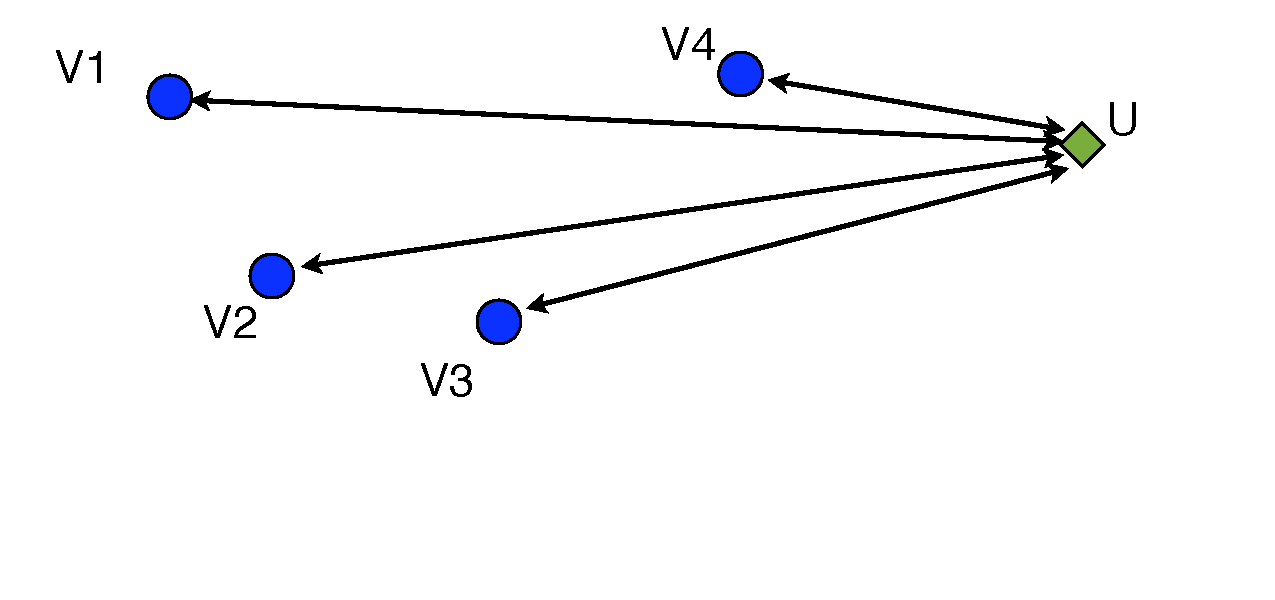
\includegraphics[height=5cm,width=10cm]{figures/divergenceAnalysis.pdf}
\pause \\
\R{$\vv^{t+1}$} is chosen to minimize \R{$\RE{\vv^{t+1}}{\vv^t}+\vv^{t+1} \cdot \boldell^t$}
\pause \\
Last line \B{is confusing!} I don't understand it!
\pause \\
But Manfred Warmuth does!
\end{frame}

\begin{frame}
\frametitle{Proof of Lemma}
\begin{itemize}
\item \R{$
\RE{\vu}{\vv^{t}} - \RE{\vu}{\vv^{t+1}} = \ell_A^t - \vu \cdot \boldell^t
$}
\item
\R{\begin{eqnarray*}
\lefteqn{\RE{\vu}{\vv^{t}} - \RE{\vu}{\vv^{t+1}}} \pause \\ 
& = & \sum_i u_i \log \frac{u_i}{v_i^t} - \sum_i u_i \log \frac{u_i}{v_i^{t+1}} \pause 
 =  \sum_i u_i \log \frac{v_i^{t+1}}{v_i^t} \pause \\
& = & \sum_i u_i \log \paren{\frac{W^t}{W^{t+1}} \; \frac{\wt{t+1}{i}}{\wt{t}{i}} } \pause \\
& = & \log \frac{W^t}{W^{t+1}} + \sum_i u_i \log e^{-\ell_i^t} \pause 
 =  \ell_A^T - \sum_i u_i \ell_i^t
\end{eqnarray*}}
\end{itemize}
\end{frame}


\iffalse
\begin{frame}
\frametitle{Using relative entropy to to express the bound}

\begin{itemize}
\item Relative Entropy:
\R{\[
\RE{\vu}{\vv}
\]}
\item Normalized weights 
\R{$v_i^t = \frac{w_i^t}{\sum_j w_j^t}$}
\item
\R{\[
\forall \vu \RE{\vu}{\vp^{t+1}} - \RE{\vu}{\vp^t} =
\ell_A^t - \vu \cdot \loss
\]}
\item For general \R{$(a,c)$}-achievable loss:
\R{\[
\forall \vu, \;\; \RE{\vu}{\vp^{t+1}} - \RE{\vu}{\vp^t}  \geq
(1/c) \ell_A^t - (a/c) \vu \cdot \boldell^t = 
\eta \ell_A^t - a \eta \vu \cdot \boldell^t
\]}
\end{itemize}
\end{frame}
\fi

\begin{frame}
\frametitle{bounding general loss using relative entropy}

\begin{itemize}
\item Suppose that loss is \R{$(a,c)$}-achievable. 
\item Achievable with Vovk algorithm, learning rate \R{$\eta=\frac{a}{c}$}
\item Let \R{$\vu$} be an \B{arbitrary} distribution vector over experts.
\item \B{Lemma}:
\R{$
\RE{\vu}{\vv^{t}} - \RE{\vu}{\vv^{t+1}} \geq \frac{1}{c} \ell_A^t - \frac{a}{c} \vu \cdot \boldell^t
$}
\item Summing over \R{$t=1,\ldots,T$} we get:
\R{$
\RE{\vu}{\vv^{1}} - \RE{\vu}{\vv^{T+1}} = \frac{1}{c} L_A - \frac{a}{c} \vu \cdot \sum_{t=1}^T \boldell^t
$}
\item
\R{$ L_A \leq \min_{\vu} \paren{a \vu \cdot \sum_{t=1}^T \boldell^t + c \RE{\vu}{\vv^{1}}}$}
\item For any mixable loss, \R{$a=1$}, using \R{$\vu = \langle 0,\ldots,0,1,0,\ldots,0
  \rangle$} and \R{$\vv^1 = \langle 1/N,\ldots,1/N \rangle$} we get the old bound:
\R{$ L_A \leq \min_i L_i + c \log N $}
\end{itemize}
\end{frame}

\section{Applications of specialists}

\begin{frame}
\frametitle{Example Application}
\begin{itemize}
\item Consider the context algorithm.
\item Let each node in the tree be a specialist.
\item Gives an inferior algorithm (regret bound is twice as large)
\item But much easier to generalize.
\end{itemize}
\end{frame}

\begin{frame}
\frametitle{Generic Example}
\begin{itemize}
\item Partition the input space. Assign each part to a specialist.
\item Use several partitions, of different fineness.
\item Can partition time in addition to space.
\item Parts do not have to be disjoint.
\item Partitions can adapt to data.
\item Your idea here...
\end{itemize}

\end{frame}

\iffalse %%%%%%%%%%%%%%%%%%%%%%%%%%%%%%%%%%%%%%%%%%%%%%%%%%%%%%%%%%%%%%%%%%

\begin{frame}
\frametitle{XXX}
\begin{itemize}
\item XXX
\end{itemize}
\end{frame}

\fi %%%%%%%%%%%%%%%%%%%%%%%%%%%%%%%%%%

\end{document}


